\chapter{Solução Proposta}\label{cap:solucao}

Uma vez que o conhecimento teórico necessário para o entendimento completo do trabalho já foi apresentado, neste capítulo será definida a solução proposta.

A solução desenvolvida consiste em um algoritmo analisa imagens de vídeo de um estacionamento descoberto e determina o número de vagas livres na imagem, além da sua localização aproximada. O sistema funciona bem em imagens de menor qualidade, mas é necessário que o vídeo adquirido seja em cores.

O trabalho se preocupa em cumprir os critérios definidos no capítulo \ref{cap:trabalhos}. Além disso, o sistema foi desenvolvido de forma que pudesse processar as imagens adquiridas de forma mais próxima possível do tempo real, causando o mínimo de atrasos para o processamento de quadros subsequentes do vídeo.

O sistema recebe como entrada um vídeo em cores capturado em um certo ângulo e um vetor de regiões de interesse no vídeo. A saída do programa a cada quadro é o número de vagas livres em cada região de interesse no vídeo.

A imagem \ref{fig:fluxograma} contém um fluxograma que mostra as etapas do processamento de cada quadro do vídeo adquirido. No decorrer deste capítulo cada um desses passo será discutido com mais detalhes.

\begin{figure}
	\centering
	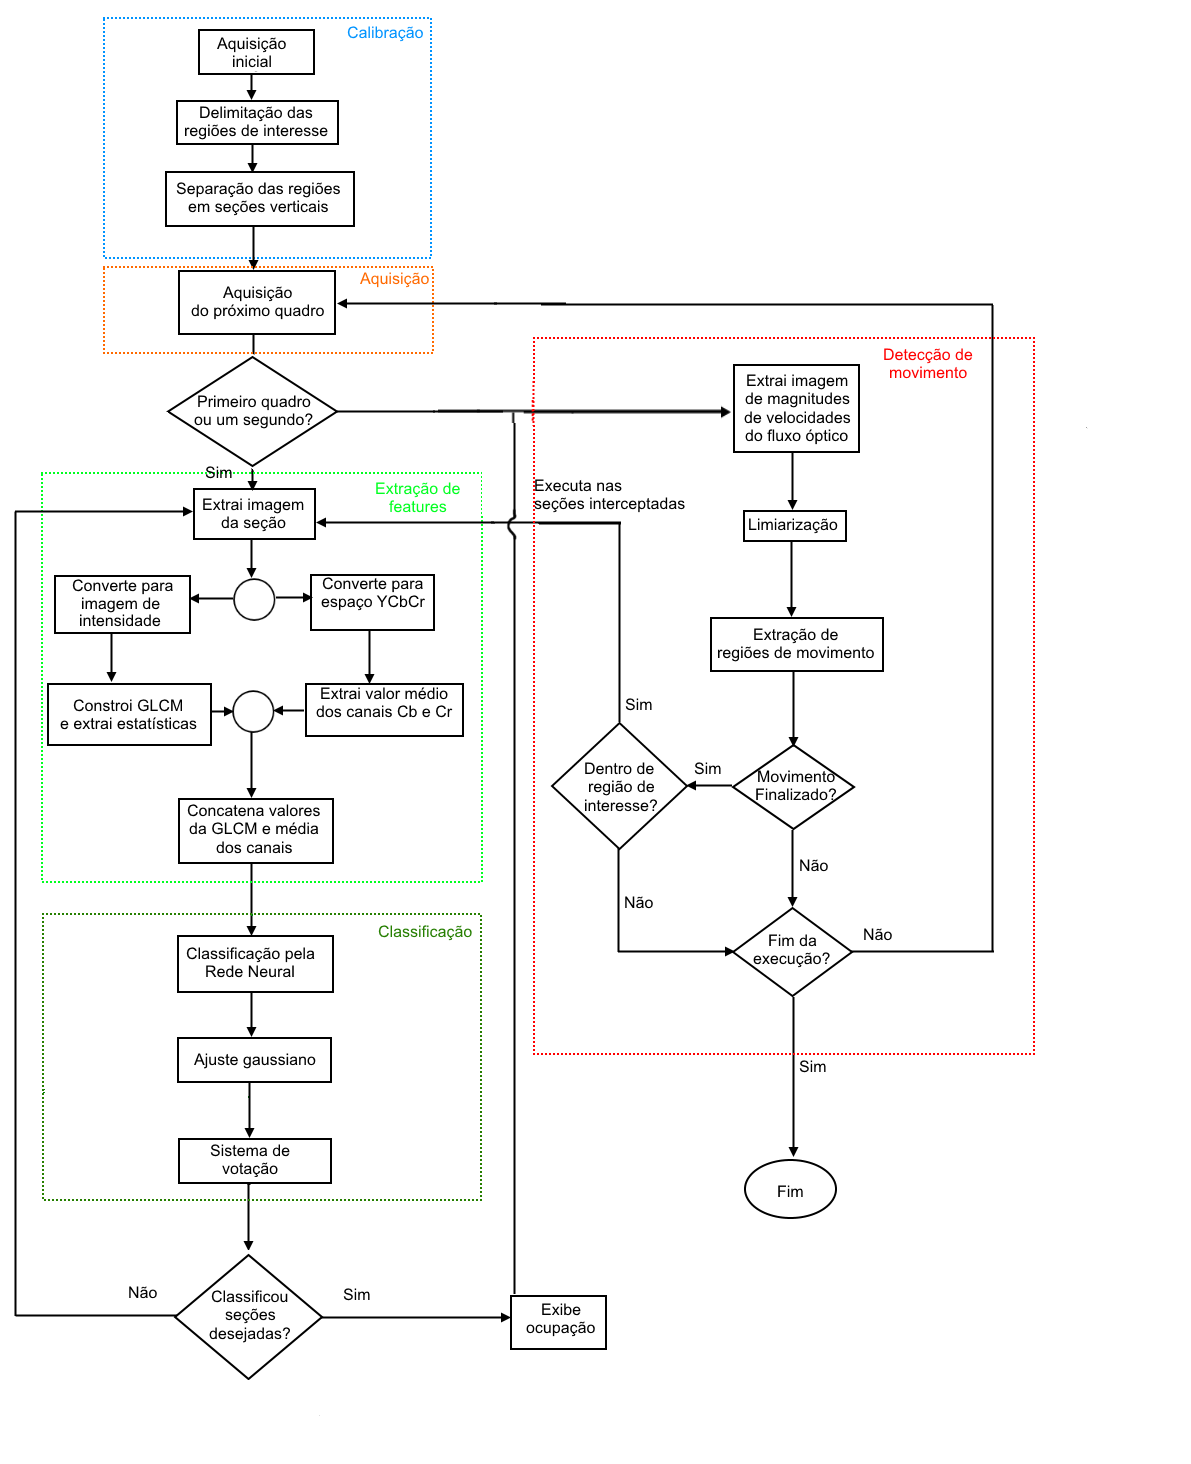
\includegraphics[width=1\textwidth]{fluxograma}
	\label{fig:fluxograma}
	\caption{Um fluxograma com o funcionamento geral do programa}
	\centering
\end{figure}



\section{Aquisição}\label{sec:aquisicao}

Uma câmera montada em um poste de luz ou outro ponto similar captura as imagens utilizadas pelo programa. A câmera é montada de forma que o seu campo de visão contenha o máximo de vagas possível, porém que ainda seja possível visualizar o asfalto das vagas desocupadas e ocorra o mínimo de oclusão de veículos. A figura \ref{fig:aquisicao} mostra um quadro de uma aquisição em ângulo ideal.

\begin{figure}[!ht]
	\centering
	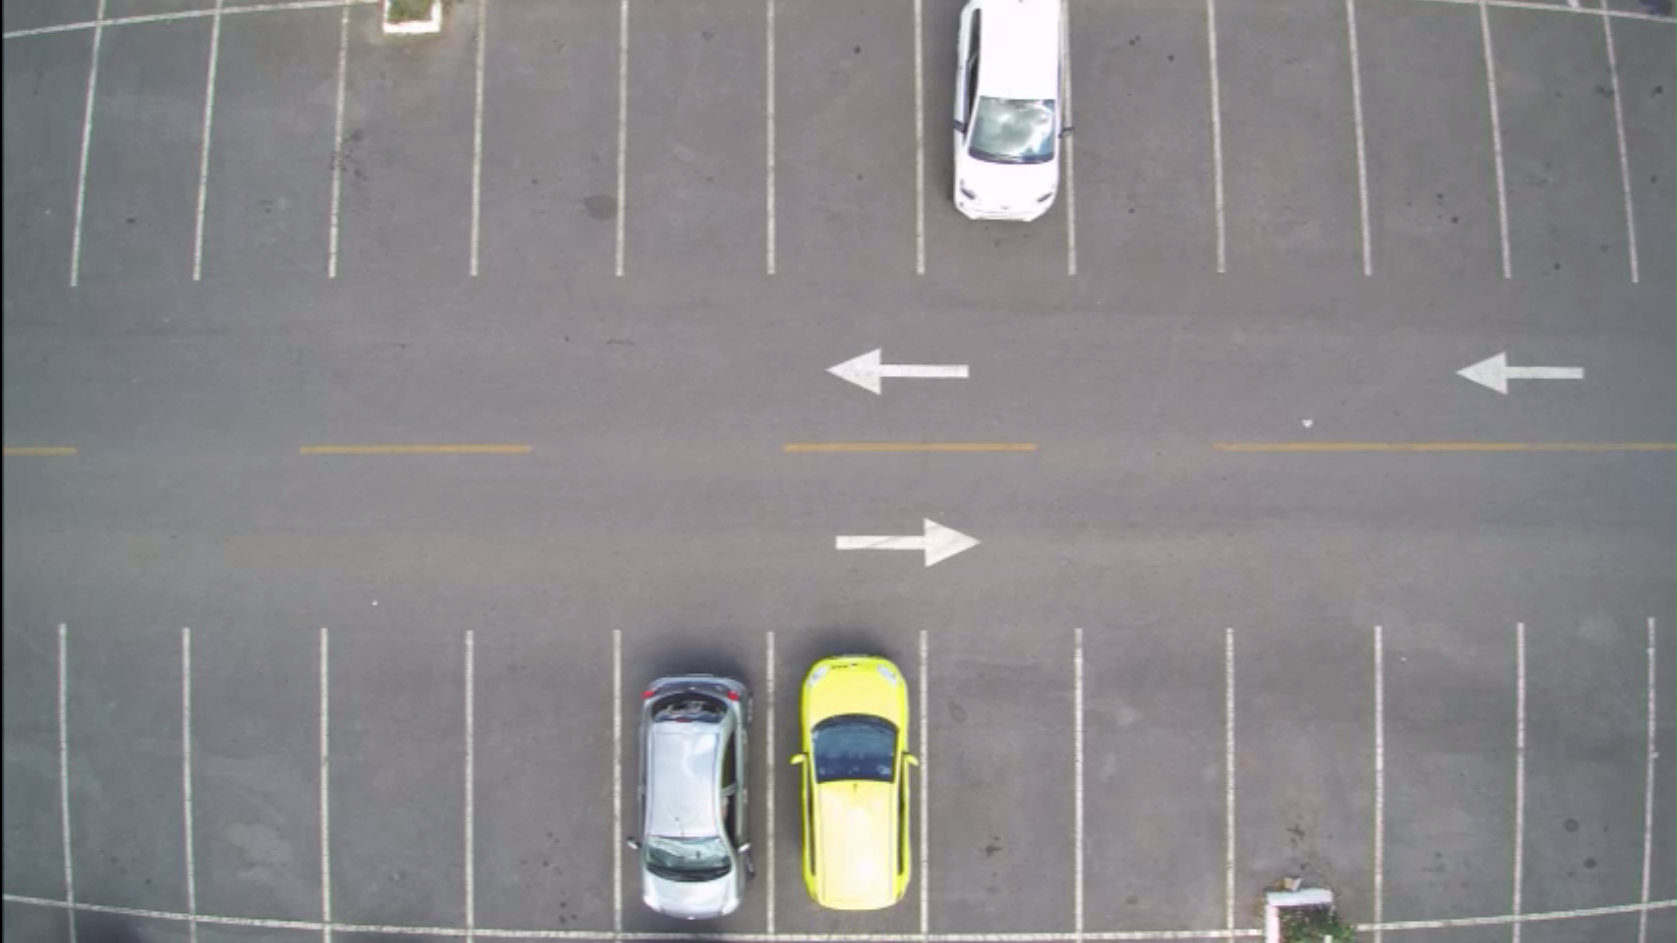
\includegraphics[width=8cm]{Vazio3}
	\label{fig:aquisicao}
	\caption{Um quadro de um vídeo adquirido por uma câmera do sistema}
	\centering
\end{figure}

Neste trabalho, a preocupação foi implementar um programa que analisa as imagens de uma única câmera de vídeo. Em uma aplicação no mundo real, diversas câmeras seriam instaladas para aumentar a cobertura do estacionamento. Neste caso, cada vídeo seria processado por uma cópia diferente do sistema, responsável pela área coberta pela câmera correspondente. As saídas de cada cópia do programa correspondem a ocupação das vagas em um setor diferente do estacionamento.

\section{Regiões de Interesse}\label{sec:ROIs}

No momento da instalação do programa, é necessário definir um número qualquer de regiões de interesse(\textit{Regions of interest} ou ROIs). Essas regiões determinam a área da imagem onde existem vagas. Além de determinar as regiões, deve-se informar ao programa o número de vagas existente em cada região de interesse.

As ROIs devem ser retangulares e determinadas de forma a não haver interseção entre elas, como exemplificado na figura \ref{fig:ROIs} que mostra as regiões determinadas para o quadro da figura \ref{fig:aquisicao}.

\begin{figure}
	\centering
	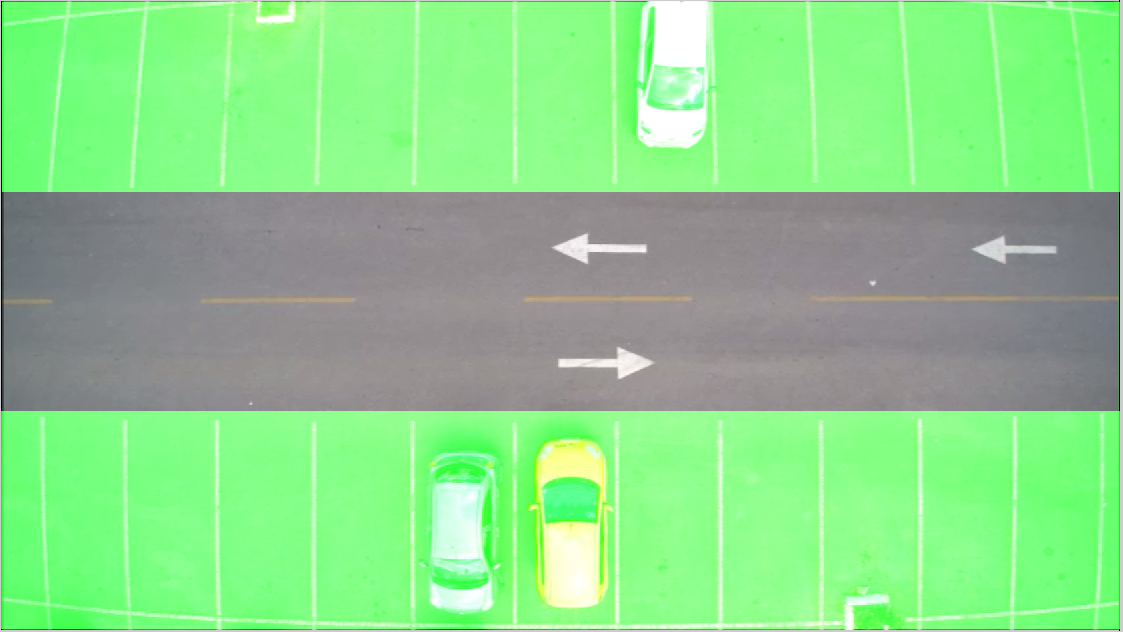
\includegraphics[width=8cm]{ROIs}
	\label{fig:ROIs}
	\caption{O mesmo quadro da figura \ref{fig:aquisicao}, depois de definidas as regiões de interesse, marcadas de verde.}
	\centering
\end{figure}

Depois de determinadas as regiões de interesse, cada uma delas é dividida em um número igual de seções verticais como ilustrado na figura \ref{fig:secoesVerticais}. Como as vagas não são determinadas individualmente no momento da instalação do programa, é necessário que seja feita alguma divisão das ROIs. Cada uma destas seções verticais é classificada separadamente em uma etapa futura do processamento. O resultado da classificação de cada seção de uma ROI determina um vetor $v$ de $n$ elementos, onde $n$ é o número de seções em que a região foi dividida e cada elemento indica a ocupação da vaga, sendo o valor $1$ correspondente a uma vaga ocupada e o valor $2$ correspondente a uma vaga livre. Através da análise deste vetor é que o programa determina o número de vagas livres em cada região. Munido do número de vagas que cada região contém e um valor aproximado do número de seções que um carro ocupa, o programa estima quantas vagas estão ocupadas, e encontra o número de vagas livres através de simples subtração e a posição aproximada destas vagas através da posição das seções livres no vetor.

\begin{figure}
	\centering
	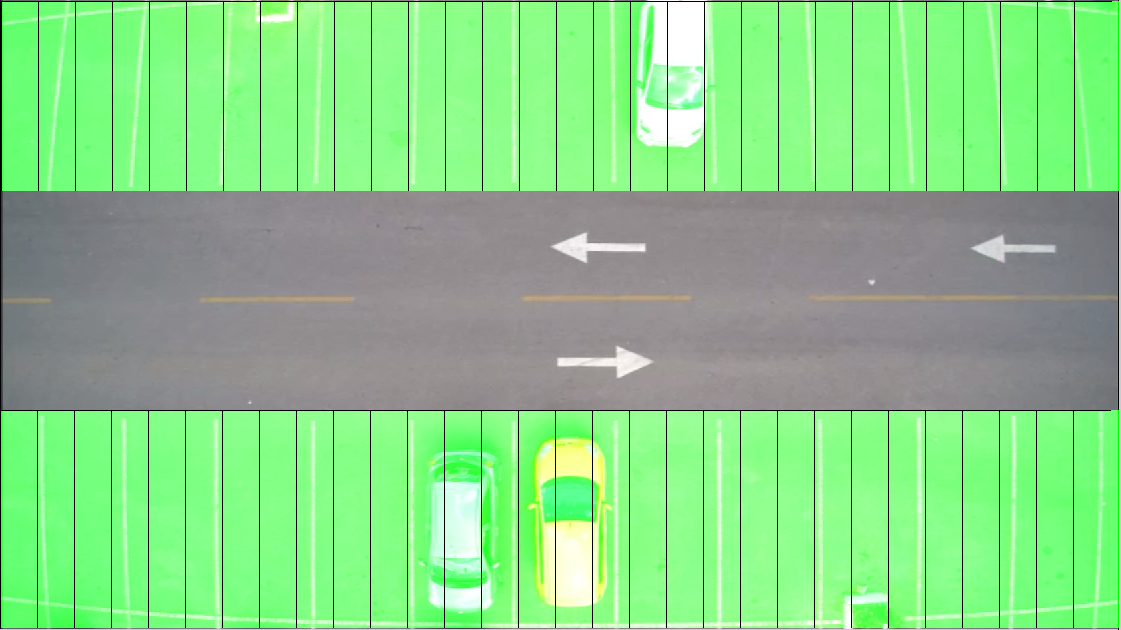
\includegraphics[width=8cm]{Secoes}
	\label{fig:secoesVerticais}
	\caption{As ROIs determinadas na figura \ref{fig:ROIs} separadas em trinta seções verticais que ainda não foram classificadas. Nesta etapa os vetores $v$ de cada região é composto de trinta valores $2$.}
	\centering
\end{figure}


Uma vez que as regiões de interesse foram definidas e divididas em seções, a etapa de calibração é finalizada e o programa pode iniciar o processo de determinação da ocupação das vagas. 

\section{Classificação das seções} \label{sec:classificacao}

O primeiro passo na execução do programa depois da calibração é a classificação de cada uma das sessões verticais criadas na imagem. Essa classificação é feita assim que a execução começa, no primeiro quadro do vídeo e é repetida a cada segundo de execução do programa. Além disso, quando se detecta movimento em uma das ROIs as sessões interceptadas pelo movimento detectada são classificadas. O processo de detecção de movimento e determinação das sessões a serem classificadas excepcionalmente é detelhado na seção \ref{sec:sub:regioesmovimento}.

Para que seja feita a extração das caracterísiticas e a classificação de uma seção, uma imagem $I_s$ é extraída do quadro de vídeo original capturado.Essa imagem corresponde à fração do quadro contida dentro dos limites da seção a ser analisada. A extração de $I_s$ consiste simplesmente em copiar os valores da matriz que representa o quadro que estavam dentro das bordas da seção em uma nova matriz de dimensões iguais às da seção. A figura \ref{fig:imgSecao} mostra um exemplo de uma $I_s$. Cada uma dessas imagens é submetida separadamente ao processo de classificação.

\begin{figure}
	\centering
	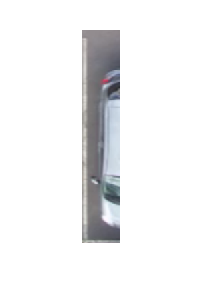
\includegraphics[height=5cm]{imgSecao}
	\label{fig:imgSecao}
	\caption{Uma imagem correspondente a uma das seções verticais definidas.}
	\centering
\end{figure}


\subsection{Extração de características}

O processo de classificação de uma seção começa com a extração das características que definem o padrão de cada classe e a criação do vetor de entrada da rede neural artifical. Dois conjuntos de características principais são extraídos: as quatro medidas extraídas da GLCM da imagem apresentadas na seção \ref{sec:GLCM} e dois valores que descrevem a crominância azul e vermelha da seção.

Para a extração da GLCM é preciso primeiro obter uma imagem de níveis de cinza que represente $I_s$. Para isso, a imagem é convertida para o espaço $YCbCr$ como descrito na seção \ref{sec:sub:ycbcr}. A imagem referente ao canal $Y$ resultante é uma imagem de intensidade e por isso é utilizada para o cálculo da GLCM. Como mencionado na seção \ref{sec:GLCM}, a construção é feita com base na vizinhança a direita de cada \textit{pixel} da imagem. Cada valor dentre os 255 possíveis é dividido dentro de 8 níveis distintos, e sempre que um valor presente em nível $N$ aparece a direita de um valor de um nível $M$, o elemento $(N,M)$ da GLCM é incrementado. A figura \ref{fig:GLCM} mostra esse processo.

Uma vez construída a GLCM referente a sessão, quatro medidas estatísticas são extraídas: contraste, correlação, energia e homogeneidade. Essas medidas são calculadas pelas equações \ref{eq:Contraste}, \ref{eq:Correlacao},\ref{eq:Energia} e \ref{eq:Homo} respectivamente. Esses valores formam um vetor $g = (contraste, correlação, energia, homogeneidade)^T$ que é parte da entrada final da rede neural artificial.

Os outros dois \textit{features} extraídos de cada sessão vêm dos canais $Cb$ e $Cr$ de $I_s$. A média de valores da matriz de cada canal é calculada através da equação \ref{eq:media}. Onde $N$ é o número total de \textit{pixels} de $I_s$ e $v_i$ é o valor do \textit{i-ésimo pixel}. Esses valores então formam o vetor $c = (M_{Cb}, M_{Cr})^T$.

\begin{equation}
	M = \frac{\sum_i=1^N v_i}{N}
\label{eq:media}
\end{equation}


Esses \textit{features} foram escolhidos por terem se mostrado suficientemente descritivos e distintivos após uma análise de um conjunto de 90 imagens. As imagens \ref{fig:histContraste},\ref{fig:histCorrelacao},\ref{fig:histEnergia},\ref{fig:histHomo},\ref{fig:histCb} e \ref{fig:histCr} mostram histogramas que descrevem a distribuição dos \textit{features} no conjunto de imagens. Em cada um dos gráficos, o eixo $x$ correspondente a valores obtidos para caracterísitica em questão e o eixo $y$ indica o número de imagens que exibiram aquele valor. As barras azuis são referentes as imagens de carros ou vagas ocupadas e as barras vermelhas referentes a vagas vazias.

\begin{figure}
	\centering
	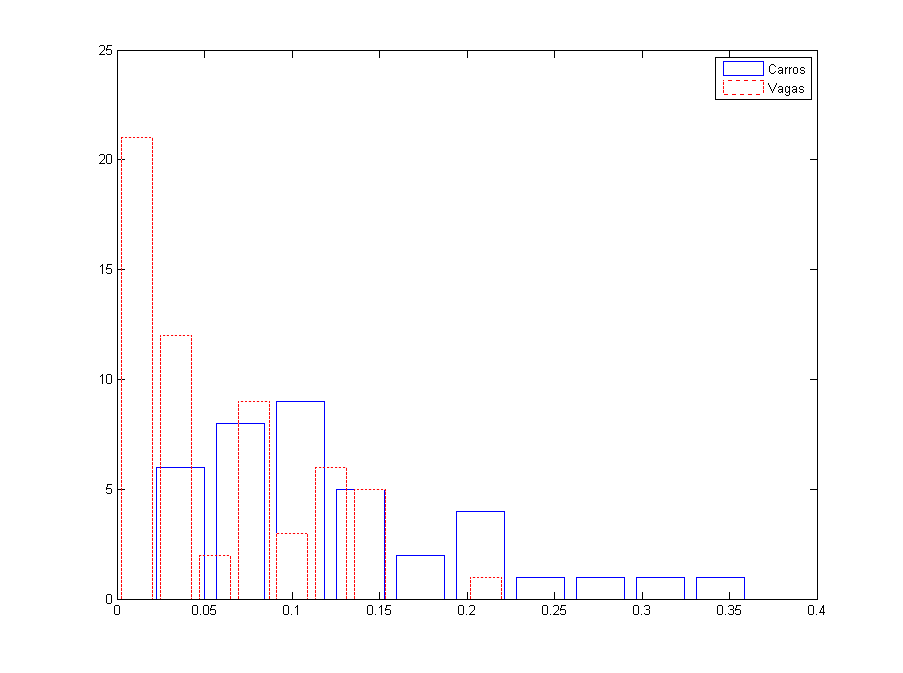
\includegraphics[width=11cm]{Contraste}
	\label{fig:histContraste}
	\caption{O histograma referente aos valores de contraste no conjunto analisado. Apesar de haver bastante sobreposição dos valores ainda é possível ver que há pouco ou nenhuma ocorrência de vagas após um certo valor.}
	\centering
\end{figure}

\begin{figure}
	\centering
	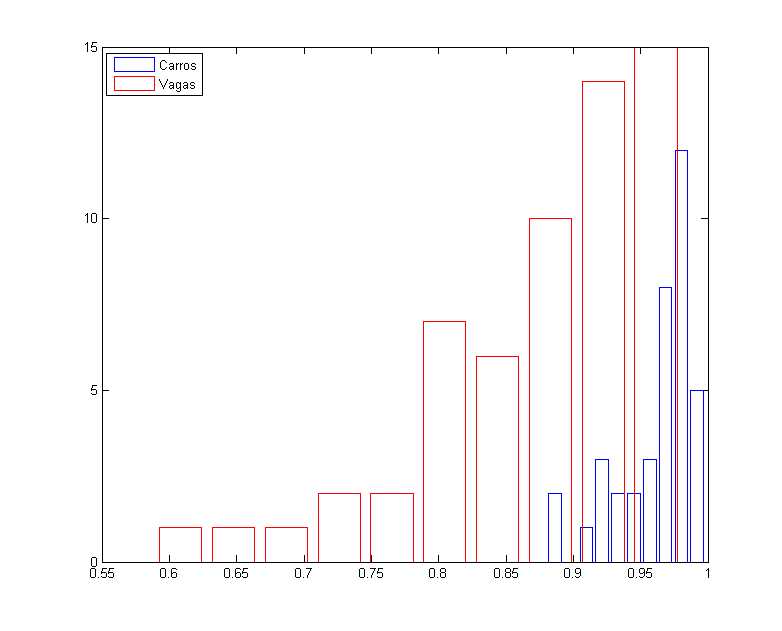
\includegraphics[width=11cm]{Correlacoes}
	\label{fig:histCorrelacao}
	\caption{O histograma referente aos valores de correlacao no conjunto analisado. Aqui é possível ver um limiar inferior para a classe dos carros. Valores abaixo deste limiar provavelmente são vagas livres.}
	\centering
\end{figure}

\begin{figure}
	\centering
	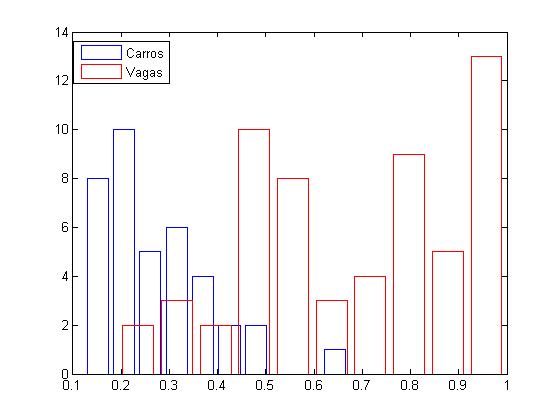
\includegraphics[width=11cm]{Energia}
	\label{fig:histEnergia}
	\caption{O histograma referente aos valores de energia no conjunto analisado. Há um ponto de divisão entre as duas classes, com pouca sobreposição de valores entre as classes.}
	\centering
\end{figure}

\begin{figure}
	\centering
	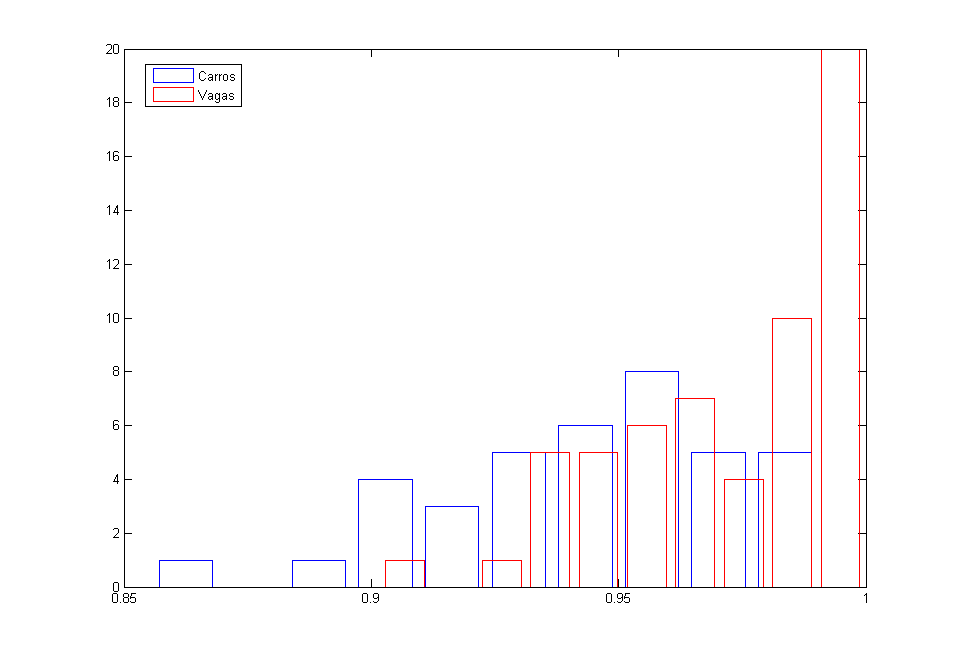
\includegraphics[width=11cm]{Homogeneidade}
	\label{fig:histHomo}
	\caption{O histograma referente aos valores de homogeneidade no conjunto analisado. Esse gráfico mostra mais sobreposição do que os anteriores, mas ainda contém bastante informação sobre a classe das vagas. }
	\centering
\end{figure}

\begin{figure}
	\centering
	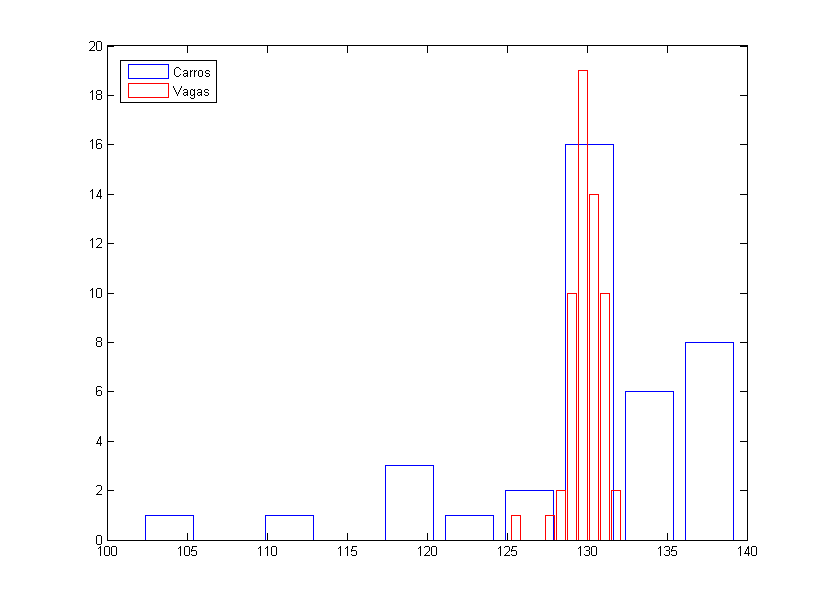
\includegraphics[width=11cm]{CrominanciaAzul}
	\label{fig:histCb}
	\caption{O histograma referente aos valores médios de crominância azul no conjunto analisado. Apesar de haver alta variedade nos valores encontrados nas imagens de carros, as imagens de faixa possuem valores médios em uma faixa estreita. }
	\centering
\end{figure}

\begin{figure}
	\centering
	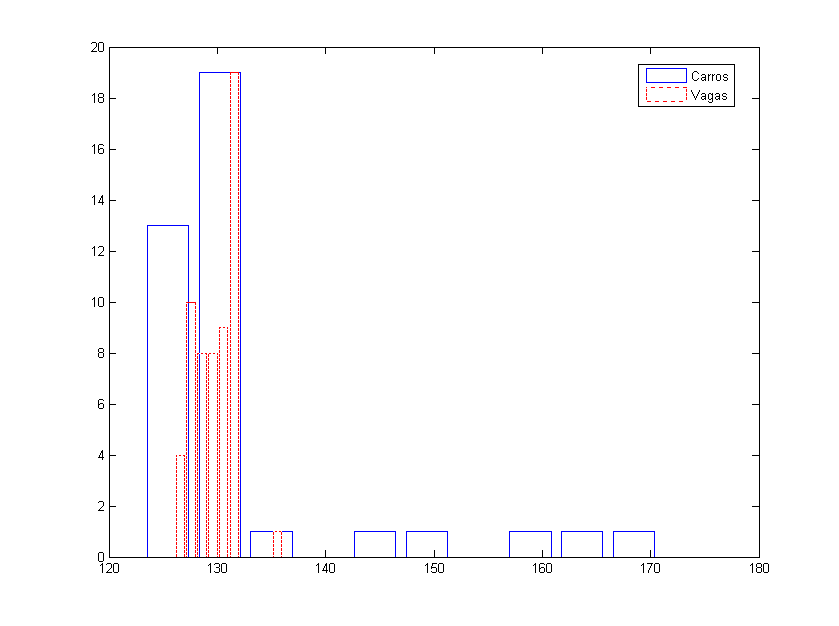
\includegraphics[width=11cm]{CrominanciaVermelha}
	\label{fig:histCr}
	\caption{O histograma referente aos valores médios de crominância vermelha no conjunto analisado, mostrando comportamento semelhante ao histograma de de valores médios de crominância azul. }
	\centering
\end{figure}


\subsection{Classificação da rede neural artificial}

\subsection{Ajuste gaussiano dos vizinhos}

\subsection{Sistema de votação}


\section{Extração do movimento}

\subsection{Fluxo Óptico}

\subsection{Regiões de movimento}\label{sec:sub:regioesmovimento}





